\documentclass[11pt]{article}
\usepackage[a4paper,margin=1in]{geometry}
\usepackage{microtype}
\usepackage{amsmath,amssymb}
\usepackage{graphicx}
\usepackage{booktabs}
\usepackage{tabularx}
\usepackage{xcolor}
\usepackage{tikz}
\usetikzlibrary{arrows.meta,positioning,fit,calc}
\usepackage[hidelinks]{hyperref}
\usepackage{caption}
\captionsetup{font=small,labelfont=bf}

\definecolor{gsblue}{HTML}{2A78D6}
\definecolor{gsgray}{HTML}{52514E}
\newcommand{\code}[1]{\texttt{#1}}
\newcommand{\prop}[1]{\textsf{#1}}

\title{GraphScout: Schema-Aligned Knowledge Graph Construction and\\Graph-Guided Question Answering with a 1.5B-Parameter Local Model}
\author{Onyeneke Sochimazuru Kenneth\\[2pt]
\small\href{mailto:mrsochimazuru@gmail.com}{\texttt{mrsochimazuru@gmail.com}}\\
\small\url{https://github.com/Sochimazuru/graphscout}}
\date{\textsc{Extended Abstract}\\[2pt]\small Proof-of-concept prepared for a PhD application\quad$\cdot$\quad October 2026}

\begin{document}
\maketitle

\begin{abstract}
I describe GraphScout, a small end-to-end pipeline that builds a knowledge graph from research abstracts with a locally run language model and answers questions by walking that graph. A 1.5B-parameter model (\code{qwen2.5:1.5b}, served by Ollama on a laptop CPU) performs open information extraction on 20 arXiv abstracts about GraphRAG and knowledge graphs. Extracted relations are aligned to a small ontology anchored to Schema.org and PROV-O, entities are merged with deterministic resolution rules, and every fact is stored in RDF with a pointer to its source paper. A three-stage agent loop (planner, explorer, answerer) answers questions over the graph, with a symbolic routing step that maps relation words in the question to schema properties. The resulting graph has 193 entities and 99 relation facts, of which 92 map to a schema property. On a random sample of 40 facts checked against their source abstracts, extraction precision is 0.625 (95\% Wilson interval 0.470 to 0.758). The errors are dominated by wrong relations, wrong subjects and garbled relation strings, with one hallucinated dataset. In a five-question case study, two answers are correct, one is partly correct and two are wrong, and none of the six answer sentences carries an inline citation. The code, data, graph and audit labels are public.
\end{abstract}

\section{Introduction}

Retrieval-augmented generation (RAG) grounds a language model in retrieved text \cite{lewis2020rag}. Retrieving isolated text chunks makes multi-hop questions hard, because the facts needed to answer them sit in different places. GraphRAG approaches organise the source material as a graph first and retrieve along its structure \cite{edge2024graphrag,han2025ragvsgraphrag}, and agent-style methods explore the graph step by step during reasoning \cite{sun2024tog,thompson2025isgraphrag,gusarov2025multiagent}.

Building the graph is the expensive part. Hand-built graphs do not scale, and automatic extraction with language models produces inconsistent names, free-form relations and occasional hallucinations. Recent work also reports that small local models struggle to produce valid structured output at all \cite{fernandes2026consumer}.

GraphScout is a compact study of that whole chain under a tight constraint: one laptop, no GPU, and a 1.5B-parameter model. The aim is a working pipeline that can be inspected end to end: every stage can be traced, and every reported number comes from a file in the repository. It makes no claim to a new state of the art. The contributions are:
\begin{itemize}
  \item an open information extraction stage with a repair step for cut-off JSON, which recovers usable output from a model that often exceeds its output budget (Section~\ref{sec:extract});
  \item schema alignment of open relations to an 11-property ontology, with rules refined from the relation wordings the model actually produced, and deterministic entity resolution (Sections~\ref{sec:align} and \ref{sec:resolve});
  \item an RDF graph in which every fact is a reified statement with PROV-O provenance (Section~\ref{sec:store});
  \item graph-guided question answering that combines symbolic relation routing with LLM-driven exploration, and reports a measured grounding signal rather than model-stated confidence (Section~\ref{sec:qa});
  \item an audit of extraction precision on a random sample, with a written reason for every fact judged incorrect (Section~\ref{sec:results}).
\end{itemize}

\section{Related work}

\paragraph{Graph-based retrieval.} Edge et al.\ build an entity graph from a corpus and summarise its communities to answer global questions \cite{edge2024graphrag}. Han et al.\ compare RAG and GraphRAG under a common protocol and find that each has distinct strengths depending on the task \cite{han2025ragvsgraphrag}. Think-on-Graph lets the model explore a knowledge graph with beam search during reasoning \cite{sun2024tog}, and Inference-Scaled GraphRAG adds sequential and parallel inference-time scaling to graph traversal \cite{thompson2025isgraphrag}. Gusarov et al.\ use several agents to translate questions into Cypher queries over labelled property graphs \cite{gusarov2025multiagent}. GraphScout's explorer follows the same idea as these step-by-step methods at a much smaller scale, and adds a symbolic routing step in front of the model.

\paragraph{Knowledge graph construction with LLMs.} Open information extraction pulls relation triples from text without a fixed relation set \cite{banko2007openie}. RAKG builds document-level graphs with retrieval-augmented extraction \cite{zhang2025rakg}, and TagRAG organises extracted knowledge into hierarchical tag chains \cite{tao2025tagrag}. Chaudhary et al.\ compare spaCy, Stanford CoreNLP-OpenIE and GraphRAG for building triples for question answering \cite{chaudhary2025fusing}. Fernandes and Kanjilal run the Microsoft GraphRAG pipeline with local models on consumer hardware and report that models below roughly 7B parameters fail to produce valid structured output reliably \cite{fernandes2026consumer}. GraphScout works below that threshold on purpose and adds output repair to cope with it.

\paragraph{Semantic Web standards.} The graph uses RDF \cite{w3c2014rdf}, is queried with SPARQL \cite{w3c2013sparql}, records provenance with PROV-O \cite{w3c2013prov}, and aligns its classes to Schema.org \cite{guha2016schemaorg}. Hogan et al.\ survey knowledge graphs more broadly \cite{hogan2021kg}.

\section{Method}

\begin{figure}[t]
\centering
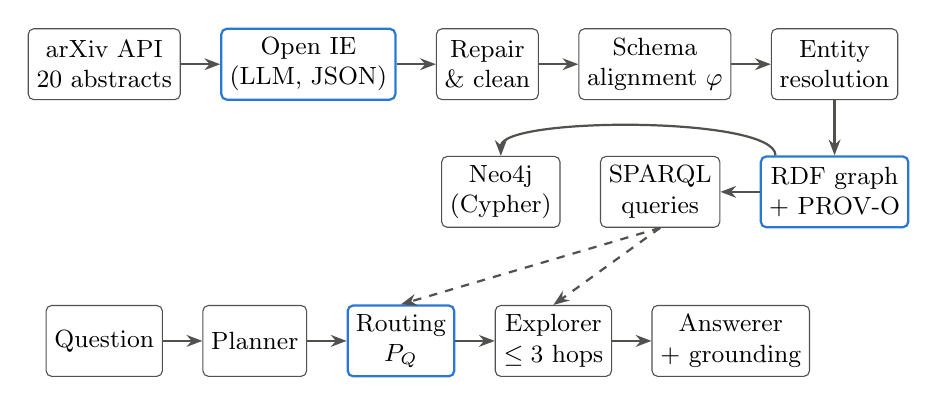
\begin{tikzpicture}[
  node distance=4mm and 5mm,
  box/.style={draw=gsgray, rounded corners=2pt, align=center, font=\small, minimum height=9mm, inner sep=3pt, fill=white},
  hl/.style={box, draw=gsblue, thick},
  arr/.style={-{Stealth[length=2mm]}, gsgray, thick}]
\node[box] (fetch) {arXiv API\\20 abstracts};
\node[hl, right=of fetch] (ext) {Open IE\\(LLM, JSON)};
\node[box, right=of ext] (rep) {Repair\\\& clean};
\node[box, right=of rep] (align) {Schema\\alignment $\varphi$};
\node[box, right=of align] (res) {Entity\\resolution};
\node[hl, below=7mm of res] (rdf) {RDF graph\\+ PROV-O};
\node[box, left=of rdf] (sparql) {SPARQL\\queries};
\node[box, left=of sparql] (neo) {Neo4j\\(Cypher)};
\node[box, below=26mm of fetch] (q) {Question};
\node[box, right=of q] (plan) {Planner};
\node[hl, right=of plan] (route) {Routing\\$P_Q$};
\node[box, right=of route] (expl) {Explorer\\$\le 3$ hops};
\node[box, right=of expl] (ans) {Answerer\\+ grounding};
\draw[arr] (fetch) -- (ext); \draw[arr] (ext) -- (rep); \draw[arr] (rep) -- (align);
\draw[arr] (align) -- (res); \draw[arr] (res) -- (rdf);
\draw[arr] (rdf) -- (sparql); \draw[arr] ($(rdf.north west)+(2mm,0)$) .. controls +(0,5mm) and +(0,5mm) .. (neo.north);
\draw[arr] (q) -- (plan); \draw[arr] (plan) -- (route); \draw[arr] (route) -- (expl);
\draw[arr] (expl) -- (ans);
\draw[arr, dashed] (sparql.south) -- (expl.north);
\draw[arr, dashed] (sparql.south) -- (route.north);
\end{tikzpicture}
\caption{GraphScout pipeline. Top: graph construction. Bottom: question answering. Routing and the explorer read the graph through SPARQL neighbour and provenance queries (dashed). Blue boxes mark the stages where the language model or the routing rules make the main decisions.}
\label{fig:pipeline}
\end{figure}

Figure~\ref{fig:pipeline} shows the pipeline. I write the graph as $\mathcal{G}=(V,E)$ with $V = V_{\mathrm{paper}} \cup V_{\mathrm{ent}}$ and labelled edges $E \subseteq V \times \mathcal{P} \times V$, where $\mathcal{P}$ is the property set defined in Section~\ref{sec:align}.

\subsection{Corpus}
The corpus is the top 20 results, by relevance, of the arXiv API query \code{abs:"GraphRAG" OR (abs:"knowledge graph" AND abs:"retrieval-augmented generation")}. Each record keeps the title, abstract, authors, date and URL. Publication dates range from January 2025 to October 2026. Only abstracts are used, which keeps extraction fast on a CPU.

\subsection{Open information extraction}\label{sec:extract}
For each abstract $d$ the model $f_\theta$ returns a set of typed entities and a set of triples,
\begin{equation}
  f_\theta(d) = \big(\mathcal{E}_d,\ \mathcal{T}_d\big),\quad
  \mathcal{E}_d \subseteq \Sigma^* \times \mathcal{C},\quad
  \mathcal{T}_d \subseteq \Sigma^* \times \Sigma^* \times \Sigma^*,\quad
  |\mathcal{E}_d|,|\mathcal{T}_d| \le 12,
\end{equation}
where $\mathcal{C}=\{\textsf{Method},\textsf{Task},\textsf{Dataset},\textsf{Metric},\textsf{Model},\textsf{Concept}\}$ and the middle element of a triple is a free-text relation. The prompt asks for canonical names, acronyms written as ``Full Name (ACR)'', and the placeholder \code{THIS\_PAPER} as subject for the paper's own contributions. Decoding uses Ollama's JSON mode with temperature 0, a 4096-token context and a hard cap of 1024 output tokens. Results are cached per paper.

\paragraph{Repairing cut-off output.} The 1.5B model can write long, repetitive JSON and hit the output cap, which leaves the text unparseable. The first paper of the run failed this way before the repair step existed. Let $x$ be the raw output and $K=\{k : x_k \in \{\texttt{\char`\}},\code{]}\}\}$ the positions just after a closing bracket. Let $\mathrm{close}(\cdot)$ append the brackets that are still open, and return nothing if the prefix ends inside a string. The repaired object is
\begin{equation}
  \hat{y} = \mathrm{parse}\big(\mathrm{close}(x_{1:k^*})\big),\qquad
  k^* = \max\{\,k \in K : \mathrm{parse}(\mathrm{close}(x_{1:k})) \neq \bot\,\}.
\end{equation}
Cutting only after a closing bracket means a half-written item is dropped, never guessed. Because decoding is deterministic, a failed parse is not retried; only network errors and server errors (HTTP 5xx) are retried.

\paragraph{Cleaning.} Names are normalised (list-shaped strings unwrapped, LaTeX markup removed) and any name that starts with a quantity, such as ``76.4\%'' or ``100 patients'', is dropped. Formally a name $n$ is discarded if it matches the regular expression \verb!^\s*\d[\d.,]*(%|\s|-|$)!. A triple whose endpoint is dropped is discarded with it.

\subsection{Schema alignment}\label{sec:align}
The ontology has the properties
\begin{equation}
\begin{aligned}
\mathcal{P} = \{&\prop{proposes}, \prop{uses}, \prop{addresses}, \prop{evaluatedOn}, \prop{measuredBy}, \prop{improves},\\
&\prop{outperforms}, \prop{comparedWith}, \prop{extends}, \prop{partOf}, \prop{reports}\} \cup \{\prop{relatedTo}\}.
\end{aligned}
\end{equation}
An ordered list of patterns $(\rho_1,p_1),\dots,(\rho_m,p_m)$ maps an open relation $r$ to a property:
\begin{equation}
  \varphi(r) = \begin{cases} p_{i^*}, & i^* = \min\{\,i : \rho_i \text{ matches } r\,\} \text{ exists},\\ \prop{relatedTo}, & \text{otherwise.}\end{cases}
\end{equation}
Order matters: \prop{outperforms} is tested before \prop{improves}, and \prop{improves} before \prop{extends}. The rules were refined by reading the relation strings of this run. For example, ``improves'' first mapped to \prop{extends}, but its objects were results such as ``factual correctness'', so I added the \prop{improves} property. When $\varphi(r)=\prop{relatedTo}$ the original wording is kept, so no information is lost. Each class in $\mathcal{C}$ is declared a subclass of a Schema.org class (for example \textsf{Dataset} $\sqsubseteq$ \code{schema:Dataset}), and papers are \code{schema:ScholarlyArticle}.

\subsection{Entity resolution}\label{sec:resolve}
Each surface name is mapped to a key $\nu(n)$ by lowercasing, replacing hyphens, removing punctuation and articles, singularising the last word, and dropping a trailing generic word (framework, approach, pipeline). Three rules propose merges:
\begin{enumerate}
  \item names with equal keys, $\nu(a)=\nu(b)$;
  \item a name written ``Full Name (ACR)'' links $\nu(\text{Full Name})$ and $\nu(\text{ACR})$;
  \item a short single-token key $b$ joins the multi-word key $a$ when $\iota(a)=b$, where $\iota$ concatenates first letters, and only if $a$ is the unique such key:
  \begin{equation}
    a \sim b \iff \iota(a) = b \ \wedge\ \big|\{a' : \iota(a') = b\}\big| = 1 .
  \end{equation}
\end{enumerate}
The merged entities are the connected components of these links, computed with union-find. A component $C$ takes the label most often used for it (preferring multi-word labels), and its type is a majority vote over the type labels $c_t$ the model gave, with ties going to a specific type over \textsf{Concept}:
\begin{equation}
  \tau(C) = \arg\max_{t \in \mathcal{C}} \big(c_t,\ \mathbb{1}[t \neq \textsf{Concept}]\big)\quad\text{(lexicographic)}.
\end{equation}

\subsection{RDF storage with provenance}\label{sec:store}
A fact is the tuple $(s,\varphi(r),o,d,r)$. Repeats of the same tuple are counted once. Each fact is written twice: as the plain triple $(s,\varphi(r),o)$ for querying, and as a reified \code{rdf:Statement} carrying \code{prov:wasDerivedFrom} $d$ and the original wording $r$. Each paper also links to every entity it mentions with \prop{mentions}. The same graph is exported as Cypher for Neo4j.

\subsection{Graph-guided question answering}\label{sec:qa}
Question answering runs in four steps.

\paragraph{Planner.} The model lists the entities named in the question $Q$. Each mention $q$ is linked to graph nodes by
\begin{equation}
  \sigma(q,n) = \begin{cases} 1, & \nu(q)=\nu(n),\\ \max\big(R(q,n),\ J(q,n)\big), & \text{otherwise,}\end{cases}
\end{equation}
\begin{equation}
  R(q,n) = \frac{2M}{|\nu(q)|+|\nu(n)|},\qquad
  J(q,n) = \frac{|W(q)\cap W(n)|}{|W(q)\cup W(n)|},
\end{equation}
where $M$ is the number of matching characters found by Python's \code{difflib} and $W(\cdot)$ is the set of words. A node is accepted if $\sigma \ge 0.88$, an exact match overrides near matches, and at most two nodes are kept per mention. If the question only names a type (``which datasets\ldots''), the start set $S$ is instead the four nodes of that type with the highest degree $\deg(v)=|\{(u,p,v)\}|+|\{(v,p,u)\}|$.

\paragraph{Routing.} A fixed table maps question words to properties, for example ``improve'' to \prop{improves} and ``compared'' to \prop{comparedWith}. With $P_Q$ the properties triggered by $Q$ and $N(S)$ the edges touching the start set, the routed evidence is
\begin{equation}
  \mathcal{E}_0 = \{\, e \in N(S) : \pi(e) \in P_Q \,\},\qquad |\mathcal{E}_0| \le 6 ,
\end{equation}
where $\pi(e)$ is the property of edge $e$. These edges enter the evidence before the model is consulted, so a small model cannot overlook them.

\paragraph{Explorer.} At hop $h$ the candidate set $\mathcal{C}_h$ holds the neighbours of the current frontier $F_h$, read with a SPARQL query. Fact edges come first; at most five \prop{mentions} edges are added, and $|\mathcal{C}_h| \le 30$. The model picks a subset $B_h \subseteq \mathcal{C}_h$ with $|B_h|\le 4$, and the frontier moves to the unvisited endpoints:
\begin{equation}
  F_{h+1} = \Big(\bigcup_{e\in B_h} \{s(e), o(e)\}\Big) \setminus \mathrm{Visited}_h,\qquad h \le 3 .
\end{equation}
Exploration stops early if the model says the evidence is enough or the frontier is empty.

\paragraph{Answerer and grounding.} The model answers from the numbered evidence only and is asked to end each sentence with the evidence it uses. Two signals are recorded. The first is the set of evidence identifiers the model says it cited, filtered to identifiers that exist. The second is measured from the answer text itself: with $\mathrm{Sent}(a)$ the sentences of answer $a$,
\begin{equation}
  u(a) = \big|\{\, x \in \mathrm{Sent}(a) : x \text{ contains no evidence identifier} \,\}\big| .
\end{equation}
Only $u(a)$ is independent of the model's own report.

\subsection{Evaluation protocol}
Extraction precision is estimated on a random sample of $n=40$ facts (fixed seed). A fact is correct only if its source abstract states it with the right direction and relation. Labels were drafted by Claude (an LLM) under this rubric and reviewed by the author, and every fact marked incorrect carries a written reason in \code{outputs/audit\_sample.csv}. With $k$ correct facts, precision is $\hat{p}=k/n$, reported with the Wilson score interval
\begin{equation}
  \frac{\hat{p} + \frac{z^2}{2n}}{1+\frac{z^2}{n}} \ \pm\ \frac{z}{1+\frac{z^2}{n}}\sqrt{\frac{\hat{p}(1-\hat{p})}{n} + \frac{z^2}{4n^2}},\qquad z = 1.96 .
\end{equation}
Schema coverage is the share of facts with $\varphi(r)\neq\prop{relatedTo}$. Question answering is assessed as a case study: I compared each answer with the source abstracts by hand.

\section{Experimental setup}
All runs used \code{qwen2.5:1.5b} \cite{qwen2024qwen25} through Ollama \cite{ollama} on a laptop CPU with no GPU, with the settings in Section~\ref{sec:extract}. Graph code uses rdflib for RDF and SPARQL, and pyvis for the interactive view. A suite of 41 unit tests with hand-written fixtures checks the plumbing (parsing, repair, alignment, resolution, routing, grounding) without calling a model. The repository includes the abstracts, the cached extractions, all outputs and the labelled audit sample, so every number below can be recomputed.

\section{Results}\label{sec:results}

\subsection{Graph}
Table~\ref{tab:graph} summarises the graph. Resolution reduced 252 entity mentions to 193 entities, and 13 repeated triples were removed. Of the 99 relation facts, 92 map to a schema property, a coverage of 0.929. Six of the seven open (\prop{relatedTo}) facts are cases where the model wrote the bare word ``on'' as the relation. Figure~\ref{fig:relations} shows the distribution over properties.

\begin{table}[t]
\centering\small
\begin{tabular}{lr}
\toprule
Quantity & Value \\
\midrule
Papers & 20 \\
Entity mentions extracted & 252 \\
Entities after resolution & 193 \\
\quad Concept / Model / Method / Task / Dataset / Metric & 89 / 26 / 25 / 19 / 18 / 16 \\
Relation facts (after removing 13 repeats) & 99 \\
Facts mapped to a schema property & 92 (0.929) \\
Triples dropped (endpoint removed by cleaning) & 2 \\
RDF triples, including ontology and provenance & 1606 \\
Neo4j export: nodes / relationships & 213 / 338 \\
\bottomrule
\end{tabular}
\caption{Graph statistics, from \code{outputs/stats.json} and \code{outputs/graph.cypher}.}
\label{tab:graph}
\end{table}

\begin{figure}[t]
\centering
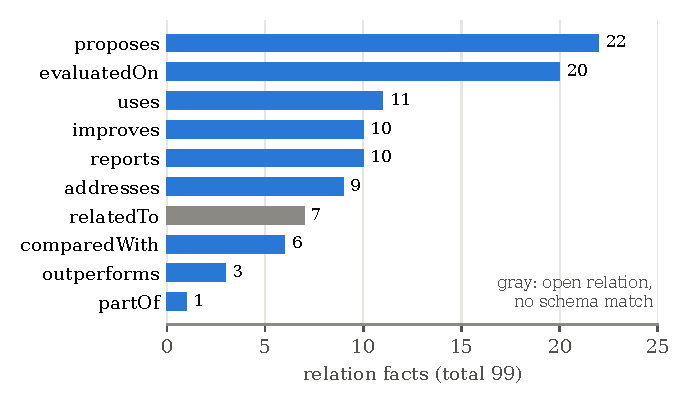
\includegraphics[width=0.72\linewidth]{figures/relations_by_property.pdf}
\caption{Relation facts per schema property. The gray bar is the open \prop{relatedTo} property, kept with its original wording.}
\label{fig:relations}
\end{figure}

Figure~\ref{fig:overview} shows the whole graph in the interactive view, and Figure~\ref{fig:detail} a zoomed region. The structure is a set of hubs, one per paper or per proposed method, with few edges between hubs. The largest hub, Graph Retrieval-Augmented Generation, is mentioned by all 20 papers, which is expected given the search query. The detail view also shows a typing error: Ollama, a serving tool, is coloured as a \textsf{Model}.

\begin{figure}[ht]
\centering
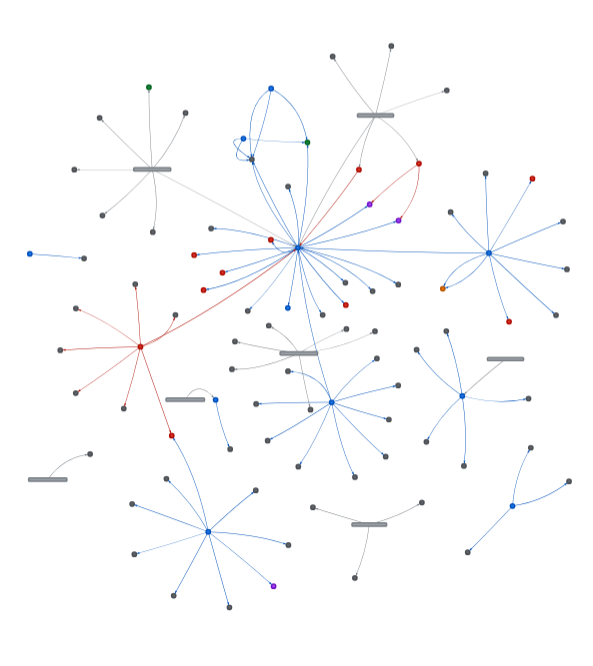
\includegraphics[width=0.48\linewidth]{figures/graph_overview.png}
\caption{The full graph in \code{outputs/graph.html}. Gray boxes are papers. Node colours: blue \textsf{Method}, orange \textsf{Task}, green \textsf{Dataset}, violet \textsf{Metric}, red \textsf{Model}, dark gray \textsf{Concept}.}
\label{fig:overview}
\end{figure}

\begin{figure}[t]
\centering
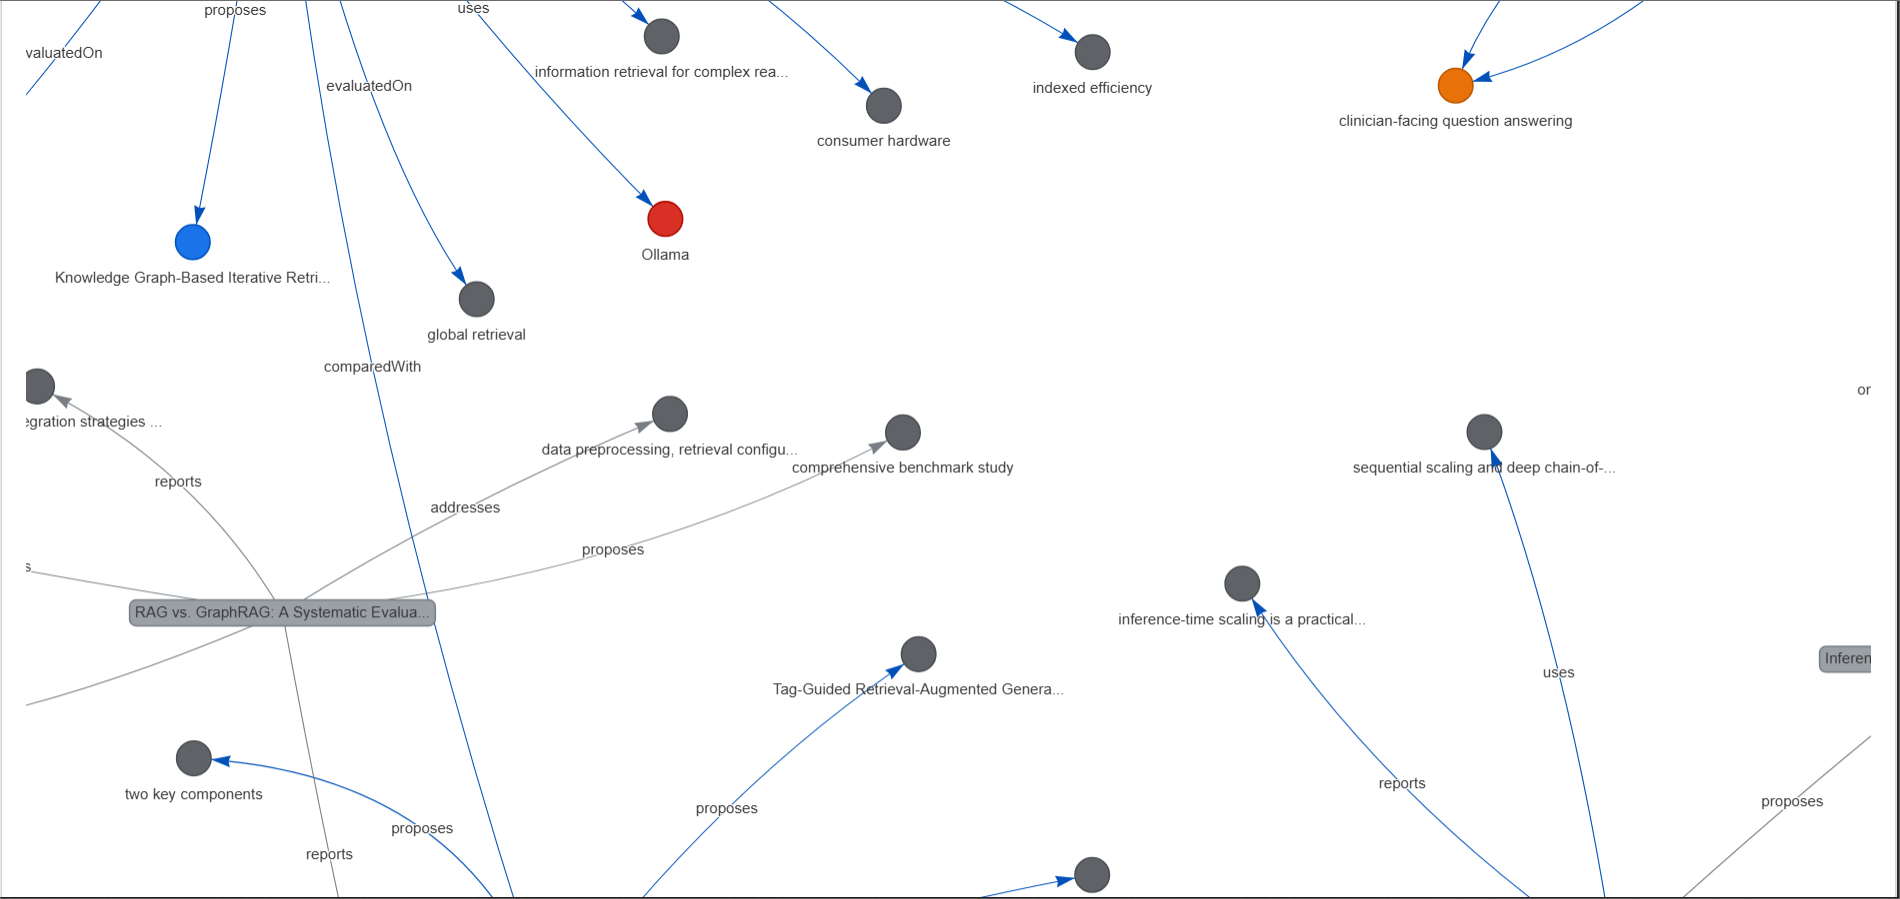
\includegraphics[width=\linewidth]{figures/graph_detail.png}
\caption{A zoomed region of the interactive graph. Edges carry schema property labels. Examples visible here include \prop{uses} to Ollama, \prop{evaluatedOn} edges from the EHR study, and the \prop{reports} and \prop{uses} edges around Inference-Scaled GraphRAG.}
\label{fig:detail}
\end{figure}

\subsection{Extraction precision}
On the 40 sampled facts, 25 are correct: $\hat{p}=0.625$, with a 95\% Wilson interval of 0.470 to 0.758. Figure~\ref{fig:errors} groups the 15 errors.

\begin{figure}[t]
\centering
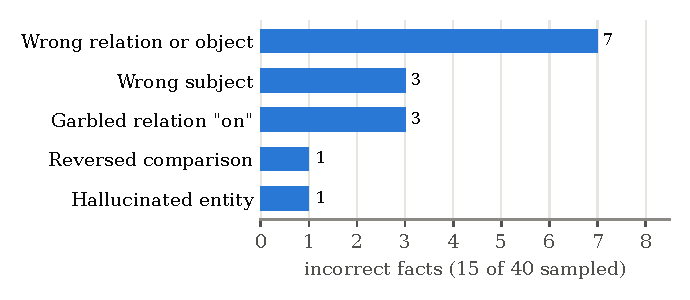
\includegraphics[width=0.72\linewidth]{figures/audit_errors.pdf}
\caption{Error types among the 15 incorrect facts in the 40-fact audit sample (\code{outputs/audit\_sample.csv}).}
\label{fig:errors}
\end{figure}

The largest group (7) is a wrong relation or object. The model wrote ``outperforms token costs'' where the paper reduces token costs, recorded a dataset (UltraDomain) as something TagRAG is compared with, and recorded an efficiency figure (``1.9x retrieval efficiency'') as a compared entity. That last case also shows a gap in the quantity filter, which does not catch numbers followed directly by ``x''. Three errors credit a method with what its paper did, for example ``GraphRAG proposes KG-IRAG'', or have a method propose itself. Three are the bare ``on'' relation. One comparison is reversed: the extracted fact says Vector RAG outperforms GraphRAG, while the abstract reports the opposite \cite{ahmad2025oran}. One entity is hallucinated: HotpotQA does not appear in the abstract it was extracted from \cite{chaudhary2025fusing}. Because that paper produced several HotpotQA facts, the hallucination spreads to every question about HotpotQA.

\subsection{Question answering}
Table~\ref{tab:qa} lists the five questions in \code{questions.txt}. Routing fired on all five. Each run used the routing step plus three exploration hops, and gathered eight or nine evidence facts.

\begin{table}[t]
\centering\small
\begin{tabularx}{\linewidth}{>{\raggedright\arraybackslash}p{4.4cm} l X}
\toprule
Question & Verdict & Note \\
\midrule
Which methods are evaluated on HotpotQA? & Wrong & Rests on the hallucinated HotpotQA facts and lists two paper titles as methods. \\
What does Inference-Scaled GraphRAG use, and what does it improve? & Correct & Both scaling strategies and the improvement in multi-hop QA match the abstract \cite{thompson2025isgraphrag}. \\
What is GraphRAG compared with, and which approach outperforms it? & Wrong & Claims GraphRAG outperforms every method listed, including BEACON-SP and TagRAG, and calls Phi-4-mini a task. Only the claim against vector RAG matches an abstract \cite{ahmad2025oran}, and the evidence it was given said the reverse. \\
What does BEACON-SP improve, and what is it compared with? & Correct & Completeness, clinical relevance and evidence grounding, against a vector RAG baseline, as in the abstract \cite{davaslioglu2026beacon}. \\
What does TagRAG compare itself with, and what does it support? & Partial & GraphRAG is right; it also lists efficiency figures and a dataset (extraction errors) and omits what TagRAG supports. \\
\bottomrule
\end{tabularx}
\caption{Question-answering case study (\code{outputs/answers.md}). Verdicts are from manual comparison with the source abstracts.}
\label{tab:qa}
\end{table}

Two answers are correct, one partly correct and two wrong. The HotpotQA answer fails because of the hallucinated extraction. The GraphRAG answer goes beyond its evidence: it was given the reversed comparison, ignored it, and claimed wins over methods that no fact links to GraphRAG in that way.

The routing step changed the BEACON-SP result. In an earlier run without routing, the explorer saw the relevant \prop{improves} and \prop{comparedWith} edges but did not select them, and the answer was incorrect. With routing, the same edges entered the evidence first and the answer matched the abstract. This is a single before-and-after observation, not a controlled comparison.

Grounding is weak. None of the six answer sentences contains an inline evidence identifier, so $u(a)$ equals the number of sentences for every answer. The model's own list of cited identifiers, by contrast, named every evidence fact for three of the five answers (nine, eight and nine facts). The self-reported list therefore says little about which facts an answer used.

\section{Discussion}
The two failure points line up with the model's size. During extraction, the 1.5B model ran past its output budget (the first paper failed this way before the repair step existed), repeated triples (13 repeats removed) and produced relation strings with no verb. Repair, cleaning and deduplication made this output usable, but they cannot fix a fact that is wrong. This matches the threshold reported by Fernandes and Kanjilal for structured output from small local models \cite{fernandes2026consumer}. In question answering, the model was a weak selector of edges and did not follow the citation format. Moving obvious decisions into deterministic steps helped: routing fixed the BEACON-SP answer, which the model alone had missed, and the citation check exposed a grounding problem that the model's own report hid.

Two lessons carry beyond this demo. First, extraction errors propagate: one hallucinated dataset in one abstract produced several wrong facts and a wrong answer downstream, and the provenance links made it quick to trace. Second, a model's report about its own citations should not be counted as grounding; a check on the answer text is cheap and more honest.

\section{Limitations}
The study is small. There is one model, one corpus of 20 abstracts and one run, and the audit covers 40 facts, so the interval on precision is wide. Recall is not measured. The question-answering results are a case study of five questions judged by hand, not a benchmark, and there is no comparison with chunk-based RAG on the same questions. Only abstracts are used; full papers, figures and tables would need a multimodal model. Schema alignment and entity resolution are rule-based and miss paraphrases.

Each limitation suggests a next step: a larger model behind the same \code{--model} flag, with the audit re-run on the same sample; a grounding filter that drops entities whose names do not appear in their source abstract (which would have caught the HotpotQA hallucination); alignment to larger ontologies such as Wikidata or the Open Research Knowledge Graph; and a multi-hop QA benchmark such as HotpotQA \cite{yang2018hotpotqa} for a proper comparison between graph exploration and plain retrieval.

\section{Conclusion}
GraphScout shows that the full chain from abstracts to a provenance-tracked RDF graph to graph-guided answers can run on a laptop CPU with a 1.5B-parameter model, and it measures where that chain breaks. Extraction precision is 0.625 on a 40-fact sample, schema coverage is 0.929, and two of five case-study answers are correct. The main sources of error are the extraction model and the answerer's handling of evidence, not the graph machinery.

\paragraph{Reproducibility.} Code, data and outputs are at\\ \url{https://github.com/Sochimazuru/graphscout}.\\ The commands below rebuild the graph, rerun the questions and recompute precision from the labelled sample:
\begin{verbatim}
python -m graphscout all
python -m graphscout ask --file questions.txt
python -m graphscout audit-score
\end{verbatim}

\begin{thebibliography}{99}\small

\bibitem{ahmad2025oran} S.~Ahmad, Z.~Nezami, M.~Hafeez, et al. Benchmarking vector, graph and hybrid retrieval augmented generation (RAG) pipelines for Open Radio Access Networks (ORAN). arXiv:2507.03608, 2025.

\bibitem{banko2007openie} M.~Banko, M.~J.~Cafarella, S.~Soderland, M.~Broadhead, and O.~Etzioni. Open information extraction from the web. In \emph{IJCAI}, 2007.

\bibitem{chaudhary2025fusing} V.~Chaudhary, N.~Soni, N.~Singh, et al. Fusing knowledge and language: A comparative study of knowledge graph-based question answering with LLMs. arXiv:2509.09272, 2025.

\bibitem{davaslioglu2026beacon} K.~Davaslioglu, N.~Conger, S.~Kompella, et al. BEACON-SP: Ontology-grounded GraphRAG framework for clinical suicide risk assessment. arXiv:2610.09026, 2026.

\bibitem{edge2024graphrag} D.~Edge, H.~Trinh, N.~Cheng, et al. From local to global: A Graph RAG approach to query-focused summarization. arXiv:2404.16130, 2024.

\bibitem{fernandes2026consumer} P.~Fernandes and R.~Kanjilal. GraphRAG on consumer hardware: Benchmarking local LLMs for healthcare EHR schema retrieval. arXiv:2605.20815, 2026.

\bibitem{guha2016schemaorg} R.~V.~Guha, D.~Brickley, and S.~Macbeth. Schema.org: Evolution of structured data on the web. \emph{Communications of the ACM}, 59(2), 2016.

\bibitem{gusarov2025multiagent} A.~Gusarov, A.~Volkova, V.~Khrulkov, et al. Multi-agent GraphRAG: A text-to-Cypher framework for labeled property graphs. arXiv:2511.08274, 2025.

\bibitem{han2025ragvsgraphrag} H.~Han, L.~Ma, Y.~Wang, et al. RAG vs.\ GraphRAG: A systematic evaluation and key insights. arXiv:2502.11371, 2025.

\bibitem{hogan2021kg} A.~Hogan, E.~Blomqvist, M.~Cochez, et al. Knowledge graphs. \emph{ACM Computing Surveys}, 54(4), 2021.

\bibitem{lewis2020rag} P.~Lewis, E.~Perez, A.~Piktus, et al. Retrieval-augmented generation for knowledge-intensive NLP tasks. In \emph{NeurIPS}, 2020.

\bibitem{ollama} Ollama. \url{https://ollama.com}.

\bibitem{qwen2024qwen25} Qwen Team. Qwen2.5 technical report. arXiv:2412.15115, 2024.

\bibitem{sun2024tog} J.~Sun, C.~Xu, L.~Tang, et al. Think-on-Graph: Deep and responsible reasoning of large language model on knowledge graph. In \emph{ICLR}, 2024.

\bibitem{tao2025tagrag} W.~Tao, X.~Li, Y.~Lan, et al. TagRAG: Tag-guided hierarchical knowledge graph retrieval-augmented generation. arXiv:2601.05254, 2025.

\bibitem{thompson2025isgraphrag} T.~Thompson, S.-H.~Lim, P.~Liu, et al. Inference scaled GraphRAG: Improving multi hop question answering on knowledge graphs. arXiv:2506.19967, 2025.

\bibitem{w3c2013prov} W3C. PROV-O: The PROV ontology. W3C Recommendation, 2013.

\bibitem{w3c2013sparql} W3C. SPARQL 1.1 query language. W3C Recommendation, 2013.

\bibitem{w3c2014rdf} W3C. RDF 1.1 concepts and abstract syntax. W3C Recommendation, 2014.

\bibitem{yang2018hotpotqa} Z.~Yang, P.~Qi, S.~Zhang, et al. HotpotQA: A dataset for diverse, explainable multi-hop question answering. In \emph{EMNLP}, 2018.

\bibitem{zhang2025rakg} H.~Zhang, J.~Si, G.~Yan, et al. RAKG: Document-level retrieval augmented knowledge graph construction. arXiv:2504.09823, 2025.

\end{thebibliography}
\end{document}
